\section{Requisitos}

En esta sección se abordarán los requisitos planteados en el paquete, tanto los iniciales como los que se han ido planteando a lo largo del desarrollo ya sean funcionales o no funcionales. 

\subsection{Requisitos Funcionales}
\begin{itemize}
    \item RF1. Como usuario puedo utilizar el editor de diálogos para crear cajas y conexiones que representen conversaciones.
    \item RF2. Como usuario puedo exportar los diálogos de forma que sean legibles por el código del juego.
    \item RF3. Como usuario puedo reproducir los diálogos en el juego.
    \item RF4. Como usuario puedo añadir etiquetas al texto para reproducir animaciones del texto.
    \item RF5. Como usuario puedo utilizar el sistema de guardado para que mi juego tenga datos persistentes.
    \item RF6. Como usuario puedo usar el sistema de carga para cargar y descargar recursos.
    \item RF7. Como usuario puedo manejar los sonidos que aparecen en mi juego a través del sistema de sonido.
    \item RF8. Como usuario puedo añadir un sistema de niveles a mi juego mediante el sistema de experiencia.
    \item RF9. Como usuario puedo insertar un personaje jugable con cámara en cualquier perspectiva.
    \item RF10. Como usuario puedo insertar un personaje jugable con movimiento basado en físicas o discreto.
    \item RF11. Como usuario puedo insertar un personaje jugable ya sea en 2D o 3D.
    \item RF12. Como usuario puedo depurar las herramientas del paquete.
    \item RF13. Como usuario puedo generar una mazmorra o un laberinto usando el generador de mazmorras.
    \item RF14. Como usuario puedo utilizar algoritmos para encontrar el camino mínimo para salir de un laberinto o llegar a la hora de una mazmorra.
    \item RF15. Como usuario puedo modificar el tamaño y posición de una mazmorra.
    \item RF16. Como usuario puedo hacer que un objeto flote y rote.
    \item RF17. Como usuario puedo añadir interacciones a mi juego.
    \item RF18. Como usuario puedo añadir vida, daño y muerte a mi juego.
    \item RF19. Como usuario puedo añadir lanzar un objeto que utilice físicas en cualquier dirección.
    \item RF20. Como usuario puedo hacer que un objeto siempre mire a cámara.
    \item RF21. Como usuario puedo utilizar curvas de animación para sacudir la cámara en 2D y 3D, para cámaras de Unity y Cinemachine.
\end{itemize}

\subsection{Requisitos No Funcionales}

\begin{itemize}
    \item RNF1. Los módulos del paquete deben ser escalables.
    \item RNF2. Los módulos del paquete deben estar documentados.
    \item RNF3. El código del paquete debe ser legible y estar bien estructurado.
    \item RNF4. El paquete debe ser usable y recibir buenos resultados en las encestas de satisfacción.
\end{itemize}

\section{Herramientas y Tecnologías}

\subsection{C\# \& Unity}

Se ha utilizado Unity\cite{unity} como motor para el que está diseñado el paquete y C\#\cite{csharp} como lenguaje de programación, se ha elegido este motor dado que era el motor público más utilizado por estudiantes y equipos pequeños y medianos.

\subsection{Visual Studio}

Visual Studio\cite{visualstudio} es un IDE y editor de código para C++ y .Net y C\#, es el editor de código por defecto de Unity y el que se ha utilizado por defecto para el desarrollo del proyecto. 

\subsection{Git \& Github}

Github\cite{github} es un entorno de desarrollo colaborativo y control de versiones web basado en la tecnología Git. Para mantener el proyecto y poder trabajar en el desde distintos equipos, se ha alojado el proyecto de del paquete\cite{Repo} en él.

\subsection{UniTask}

UniTask\cite{UniTask} es una librería que ofrece una implementación de async/await sin necesidad de alocataciones de memoria basada en estructuras. Se ha aprovechado esta librería para la implementación del sistema de carga de escenas, ya que permite un funcionamiento asíncrono.

\section{Arquitectura y Análisis}
En la siguiente sección se detallan los detalles técnicos acerca del paquete, explicando los detalles de implementación de las distintas secciones, módulos y componentes.

\subsection{Sistema de Diálogos}
aaa

\subsection{Sistema de Experiencia}
El sistema de experiencia es un pequeño conjunto de clases que permite definir una lista de niveles de 'minLevel' a 'maxLevel' dada una función lineal, cuadrática, cúbica o 
 parabólica, este sistema permite definir callbacks para eventos de subida de nivel, aumento de experiencia y llegada al nivel máximo. El sistema gestiona automáticamente las
 subidas y el aumento de experiencia y dispone de funciones de acceso para obtener los datos actualizados en cualquier momento dado.

El sistema también cuenta con la posibilidad de crear ScriptableObjects de tipo 'ExperienceMobAsset', que permiten definir la cantidad de experiencia que proporciona un evento 
 concreto, para ejemplificarlo se puede asumir que se estaría hablando de derrotar un enemigo en un juego de rol tradicional. El sistema cuenta con un manager singleton que 
 permite calcular el valor de la experiencia que daría un evento o 'Mob' concreto, además cuenta con la funcionalidad para definir distintos tipos de contextos modificadores 
 de experiencia.


\subsection{Sistema de Audio}
El sistema de audio o Audio Manager en código es una clase de tipo Singleton que permite definir una serie de ScriptableObjects de tipo 'Sound'. Estos permiten a su vez que 
se les asigne un clip de audio y una serie de parámetros como si es un efecto de sonido o una canción, un modificador de volumen, de tono o si se desea que dicho sonido 
se reproduzca en bucle. La clase Audio Manager contiene a su vez un array de 'Sounds' y es capaz de reproducir, pausar, parar o reanudar cualquier sonido o canción que contenga. 
La clase tiene también la capacidad de gestionar una lista de música aleatoria de ambiente para ese tipo de juegos. El sistema tiene capacidad para separar los distintos tipos de 
sonido, música o efecto, en distintas pistas de audio con el fin de poder ajustar los dsitintos volúmenes por separado.    

\subsection{Sistema de Guardado}
El sistema de guardado está compuesto por tres clases llamadas: 'SaveDataHandler', 'SaveDataFileHandler' y 'SaveData'. 'SaveDataHandler' es una clase de tipo Singleton que 
sirve como API para gestionar las llamadas al guardado, creación de nuevos archivos de guardado u operaciones de borrado y copia de estos. El 'SaveDataFileHandler' es por 
otra parte el encargado de gestionar la conversión de datos en memoria dinámica a archivos .json almacenados en memoria estática del dispositivo. La clase 'SaveData' por últimos
es la clase en la que se almacenan los datos que se quieran guardar. El sistema soporta guardar tipos de datos alfanuméricos, listas y diccionarios de tipo 
'SerializableDictionary', dado que los diccionarios de C\# estándar no se pueden serializar a formato JSON. La implementación del 'SerializableDictionary' es muy sencilla, 
simplemente funciona como una lista de listas de tipo 'KeyValuePair', que a su vez contienen su respectiva clave y valor. Adicionalmente el sistema permite encriptar la 
partida guardada con una sencilla función de hash de XOR, de forma que no se almacene como texto en claro en el dispositivo.  

\begin{figure}[H]
  \centering
    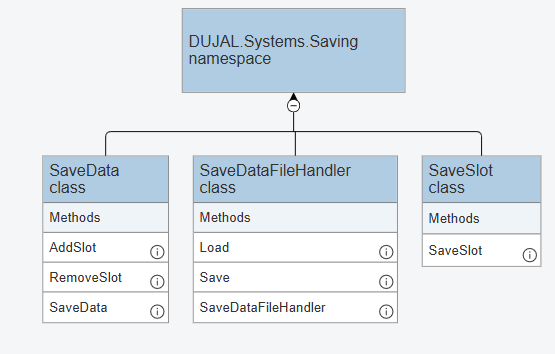
\includegraphics[width=350px,clip=true]{Saving.png}
  \caption{Diagrama de clases del Sistema de Guardado}
  \label{fig:savinguml}
\end{figure}

\subsection{Sistema de Gestión Carga de Escenas}
El sistema de gestión de carga de escenas permite cargar de forma asíncrona y sustitutiva distntas escenas de un proyecto. El sistema automáticamente muestra una 
pantalla de carga que también esconde automáticamente una vez termina de cargar. La pantalla de carga puede mostrar opcionalmente el progreso de la carga. Añadir una nueva
 escena pasa, aparte de por añadir una nueva escena a las dependencias del proyecto en unity, por añadir un nuevo valor al enumerado de la clase 'SceneIndex'. Dicha clase 
 permite operar con 'SceneIndex' intercambiablemente como objetos, enumerados o enteros.

\subsection{Herramienta de Dibujado de Colisiones 2D}
aaa

\subsection{Herramienta de Cuadrícula}
aaa

\subsection{Generador de Mazmorras}
aaa

\subsection{Floater}
aaa

\subsection{Componente de Vida}
aaa

\subsection{Componente de Interacción}
aaa

\subsection{LaunchRigidbody}
aaa

\subsection{Componente de Sacudida de Cámara}
aaa

\subsection{Componente de Movimiento 2D Lateral o 'Side Scroll'}
aaa

\subsection{Componente de Movimiento 2D Cenital o 'Top Down'}
aaa

\subsection{Componente de Movimiento 3D Primera Persona o ¡First Person'}
aaa

\subsection{Componente de Movimiento 3D Tercera Persona o 'Third Person'}
aaa

\subsection{Componente de Movimiento 3D Lateral o 'Side Scroll'}
aaa

\begin{mypython}[caption={Ejemplo de código utilizado para definir la animación de 'Wobble' en el texto.},label={alg:wobbleAnimation}]
    foreach (EffectInstance effect in effects) 
    {
        for (int i = effect.TextStartIdx; i < effect.GetTextEndIndex(); ++i)
        {
            var charInfo = animationHandler.TextInfo.characterInfo[i];
            if (!charInfo.isVisible)
            {
                continue;
            }
            
            var meshInfo = animationHandler.TextInfo.meshInfo[charInfo.materialReferenceIndex];
            var verts = meshInfo.vertices;
            for (int j = 0; j < 4; ++j)
            {
                int vertexIdx = charInfo.vertexIndex + j;
                float newOrigY = Mathf.Sin(Time.time * _speed[effectIdx] + verts[vertexIdx].x * 0.01f) * _amplitude[effectIdx];
                verts[vertexIdx] = verts[vertexIdx] + new Vector3(0f, newOrigY, 0f);
            }
        }
        effectIdx++;
    }
\end{mypython}

\section{Niveles de Prueba}


\section{Documentación}
